\part{Apéndices}
\appendix

\section{Diagramas de bloque}
Son usados para modelar interacción entre procesos. Cada proceso es representado como un bloque con círculos en su perímetro que indican las acciones visibles desde el entorno.
\begin{figure}[h]
\centering
	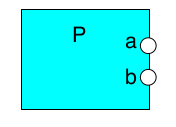
\includegraphics[scale=0.5]{imagenes/bloque_proceso}
	\caption{Proceso P con alfabeto \{a,b\}}
\end{figure}

La composición en paralelo de dos procesos se representa uniendo dos bloques con líneas entre las acciones que deben sincronizar (y si se necesita un renombre, sobre las líneas marcar el nombre de la acción).

\begin{figure}[h]
\centering
	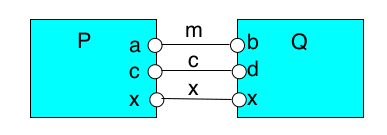
\includegraphics[scale=0.5]{imagenes/bloque_composicion}
	\caption{Compocisión de los procesos P y Q con renombre de acciones (P$||$Q) /\{m/a, m/b, c/d\}}
\end{figure}

Y el proceso $||$S que solo muestra ciertas acciones de la interacción, se representa encerrando la figura anterior dentro de otro proceso:

\begin{figure}[h]
\centering
	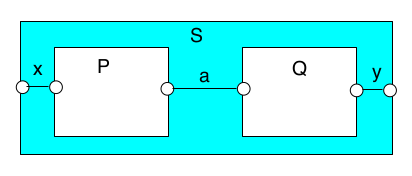
\includegraphics[scale=0.5]{imagenes/bloque-proceso-compuesto}
	\caption{Proceso S conseguido a partir de la compocisión de los procesos ConversationsP y Q: $||$S = (P$||$Q) @ \{x,y\}}
\end{figure}
